\section{Development process and implementation}
\label{chap:development_process}

This chapter details the steps used during the development of the program.
We started by re-implementing most of the code used in the previous exercise, only this time in C.
In addition we set up a timer, which was to be used for interacting with the DAC.

% - setting up interrupts from c
% - embedding assembly

\subsection{Setting up the DAC}

To get sound playing on the board, we had to use the DAC, a Digital-to-Analog Converter.
A timer was needed to be able to continuously write sound samples to the DAC.

\subsection{Timer}

The timer clock frequency is 14MHz, but for the music we only want a freqency of 44100KHz.
Therefore we set the sample period to $ \frac{\SI{14}{\mega\hertz}}{\SI{44100}{\kilo\hertz}} \approx 317 $.
This will ensure the timer interrupt is triggered 44100 times a second.

\subsection{Sound synthesis}
The three sound effects we've implemented are all generated in real-time on the board.
We made three different sound effects: a coin blip, a laser, and a level-up sound.
They are all based on a simple waveform, either a square wave or a sawtooth.
Each sound has parameters that are allowed to change for each playback.
Those parameters include frequency, slide, and ADSR parameters.
To leverage the fact that the sound samples are generated on-the-fly, we added a bit of randomization to the ADSR parameters.
This made each playback of a sound effect unique, so each time you press the button for a given sound effect it will sound slightly different.
In addition to varying the ADSR parameters, the frequency was randomized within a given interval for each of the sound effects.
We also added a custom slide to each of them – this allowed the frequency to change gradually during the sound.

\subsubsection{ADSR}

A waveform with constant frequency alone would not provide the sound effects we wanted. We therefore implemented a ADSR envelope \cite{adsr}.
The envelope consists of an attack period, a decay period, a sustain level and a release period, as seen in figure \ref{fig:adsr_envelope}.

\begin{itemize}
    \item The attack periode is the time to use from zero to maximum amplitude.
    \item The decay is the time from max amplitude down to the sustain level.
    \item The sustain level is the amplitude to rest on between the decay and release periods.
    \item The release indicates how much time to spend fading from the sustain level to zero volume.
\end{itemize}

\begin{figure}[ht!]
    \begin{center}
    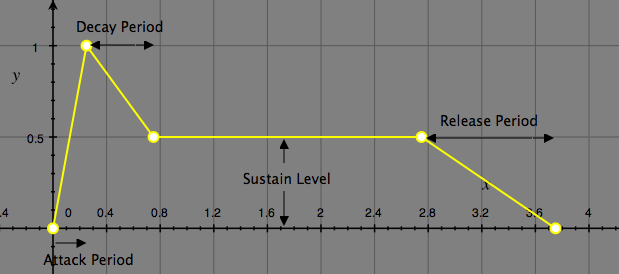
\includegraphics[width=0.8\textwidth]{assets/img/adsr.png}
    \caption{A ADSR envelope}
    \label{fig:adsr_envelope}
    \end{center}
\end{figure}

\subsubsection{Effects}

The parameter intervals for the three implemented sound effects can be seen in Table \ref{tab:sound_effects}.

\begin{table}[ht!]
    \begin{center}
    \begin{tabular}{r|lll}
    Parameter           & Coin       & Laser             & Level-up   \\
    \hline
    Waveform            & Square     & Square / Sawtooth & Sawtooth   \\
    Frequency (initial) & 1500-3000  & 1200-3200         & 100-1100   \\
    Slide               & 0          & -2                & 6          \\
    Attack              & 0          & 0                 & 0-500      \\
    Decay               & 0-3500     & 1000-3000         & 1000-3000  \\
    Sustain level       & 30-80      & 0-50              & 50-100     \\
    Release             & 4000-18000 & 4500-10500        & 2500-16500 \\
    \end{tabular}
    \end{center}
    \caption{Parameter intervals for the implemented sound effects}
    \label{tab:sound_effects}
\end{table}

All sound effect calculations are done with integers, to ensure that the calculations are fast enough to be processed within one timer interval.

\newpage

\subsubsection{Custom random function}

There was no rand() function available, so we made one ourselves:
\\[0.5cm]
\begin{code}

static unsigned int next = 1;

int rand_r(unsigned int *seed) {
    *seed = *seed * 1103515245 + 12345;
    return (*seed % ((unsigned int)RAND_MAX + 1));
}

int rand() {
    return (rand_r(&next));
}


\end{code}

\subsection{Pre-recorded melody}

% Details of exporting from FL Studio, convert to C array

\subsection{Button control}

Buttons are set up to control one sound effect each. The remaining buttons will stop the sound currently playing.
